\textcolor{red}{This chapter covers three areas: analysis of the data; discussion of the results of the analysis; and how your findings relate to the literature. The analysis of the data can be discussed here but the details of any analysis, such as statistical calculations, should be shown in the appendices. You should present any discussion clearly and logically and it should be relevant to your research questions/hypotheses or aims and objectives. Insert any tables or figures that you decide are important in a relevant part of the text not in the appendices, and discuss them fully. Make sure that you relate the findings of your primary research to your literature review. You can do this by comparison: discussing similarities and particularly differences. If you think your findings have confirmed some literature findings, say so and say why. If you think your findings are at variance with the literature, say so and say why.}
\section{Results}
Lorem ipsum dolor sit amet, consectetur adipiscing elit. Duis ut ipsum nec orci interdum sollicitudin ut eu nunc. Pellentesque ultricies eros in justo sagittis, eget blandit velit aliquet. Aenean ac lectus nibh. Quisque ac est pellentesque, ullamcorper sem sit amet, pharetra quam. Morbi ullamcorper placerat diam, sed tincidunt odio.

\textcolor{red}{When placing tables (\autoref{tab:econ}) within the body of the text, the citation is placed above the table.} 

\begin{table}[!ht]
  \centering
  {\small {\it \caption{The economic argument \label{tab:econ} \hcite{econ}}}}
  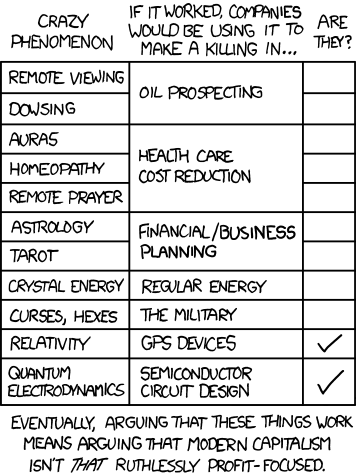
\includegraphics [scale=0.5]{Images/the_economic_argument.png} \\
\end{table}

\vfill

\newpage 

\section{Discussion}
Lorem ipsum dolor sit amet, consectetur adipiscing elit. Duis ut ipsum nec orci interdum sollicitudin ut eu nunc. Pellentesque ultricies eros in justo sagittis, eget blandit velit aliquet. Aenean ac lectus nibh. Quisque ac est pellentesque, ullamcorper sem sit amet, pharetra quam. Morbi ullamcorper placerat diam, sed tincidunt odio.

\textcolor{red}{When placing figures (illustrations, pictures, graphs, diagrams, charts, maps etc.) within the body of the text, the citation is placed below the figure (\autoref{fig:moun})}

\begin{figure}[!h]
  \centering
  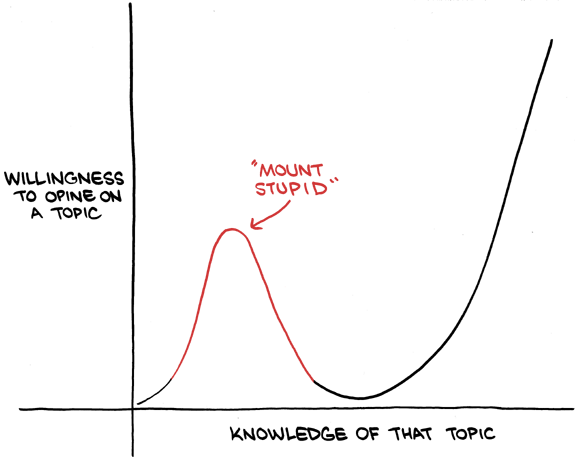
\includegraphics [scale=0.5]{Images/dunning_kruger.png} \\
  {\small {\it \caption{Dunning–Kruger effect \label{fig:moun} \hcite{mount}}}}
\end{figure}